\documentclass[a4paper,12pt]{article}
\usepackage[hmargin=2.5cm,vmargin=2.5cm]{geometry}

\usepackage[utf8]{inputenc}   % le fichier .tex est en UTF-8     
\usepackage[francais]{babel}  %typo française                    
\usepackage[T1]{fontenc}      % encodage des fonts latex         
\usepackage{lmodern}                                             
\usepackage{microtype}        % typo supplémentaires             


\usepackage{multirow}  %  pour des tableaux multilignes/multicolonnes

\usepackage{graphicx} %inclusion de graphiques

\usepackage{hyperref} % liens dans le pdf
\hypersetup{%
  pdftitle={Title},
  pdfauthor={Author1, Author2},
  pdfkeywords={keywords}
  pdfsubject={article},
  colorlinks=true,
  linkcolor=black,
  urlcolor=black,
  citecolor=black
}




\begin{document}

   \section{Les protocoles} 
    
    \begin{table}[!htbp]
      \centering

      \begin{tabular}{|l|l|r|r|c|c|}

        \hline
        Nom & Temp & Traj & Cycles  & Voisin & Proba \\
        \hline
        p1   & 0.001 &  3000000  &  1000  & 10 & 0; 1; 0.1; 0   \\      
        p2   & 0.1   &  3000000  &  1000  & 10 & 0; 1; 0.1; 0   \\  
        p3   & 0.2   &  3000000  &  1000  & 10 & 0; 1; 0.1; 0   \\ 
        p4   & 0.3   &  3000000  &  1000  & 10 & 0; 1; 0.1; 0   \\               
        p5   & 0.5   &  3000000  &  1000  & 10 & 0; 1; 0.1; 0   \\  
        p6   & 0.7   &  3000000  &  1000  & 10 & 0; 1; 0.1; 0   \\  
        p22  & 0.1   &  6000000  &  1000  & 10 & 1; 1;   1; 1   \\  
        p32  & 0.2   &  6000000  &  1000  & 10 & 0; 1; 0.1; 0   \\      
        p33  & 0.2   &  3000000  & 10000  & 10 & 0; 1; 0.1; 0   \\   
        p52  & 0.5   & 10000000  &   100  & 20 & 0; 1;   0; 1   \\  \hline   

        
      \end{tabular}      
      \caption{Les protocoles}
      \label{tab_proto}      
    \end{table}

    \section{MC et Superfamily}

    \begin{table}[!htbp]
      \centering

      \begin{tabular}{|c|r|r|r|r|r|r|}

        \hline
         & 0.001 & 0.1 & 0.2  & 0.3 & 0.5 & 0.7  \\
        \hline
        1ABO & 7382  & 8374 & 6764 & 5033 & 2576  & 1255  \\      
        1CKA & 8045  & 8497 & 9139 & 9534 & 8060  & 2490  \\  
        1BM2 & 8073  & 8002 & 6861 & 7869 & 4458  & 2821  \\  
        1M61 & 9489  & 9662 & 9825 & 9777 & 9822  & 8744  \\  
        1O4C & 7124  & 7702 & 6909 & 7849 & 7623  & 4847  \\  
        1G9O & 10000 & 10000 & 10000 & 10000 & 10000  & 9942 \\  
        1R6J & 9878  & 9871 & 9796 & 8794 & 5387 & 3787 \\  \hline
        
      \end{tabular}
      
      \caption{Résultats Superfamily selon la température (les protocoles p1 à p7).}      
      \label{tab_temp}

    \end{table}



    \section{MC et identite de sequences}


    \begin{table}[!htbp]
      \centering
      
      \begin{tabular}{|c|c|c|c|c|c|c|}
      
        \hline
        & 0.001 & 0.1 & 0.2  & 0.3 & 0.5 & 0.7  \\
        \hline
        1ABO & 33 & 33 & 33 & 32 & 32  & 30 \\      
        1CKA & 26 & 27 & 27 & 27 & 26  & 26 \\  
        1BM2 & 26 & 27 & 27 & 28 & 25  & 23 \\  
        1M61 & 40 & 41 & 41 & 41 & 41  & 39 \\  
        1O4C & 21 & 21 & 21 & 21 & 20  & 19 \\  
        1G9O & 35 & 35 & 36 & 37 & 36  & 33 \\  
        1R6J & 33 & 33 & 32 & 32 & 31  & 29 \\  \hline
        
      \end{tabular}
      

      \caption{Pourcentage d'identité de sequences selon la température.}      
      \label{tab_ident}
    \end{table}


\section{MC et meilleur energie proteus}

    \begin{table}[!htbp]
      \centering


      \begin{tabular}{|c|c|c|c|c|c|c|}

     
        \hline
         & 0.001 & 0.1 & 0.2  & 0.3 & 0.5 & 0.7  \\
        \hline
        1ABO & -270.58 & -270.13 & -270.47 & -271.66 & -281.05  & -289.79 \\      
        1CKA & -251.45 & -247.66 & -252.13 & -252.34 & -261.41  & -267.37 \\  
        1BM2 & -482.39 & -486.53 & -483.38 & -486.71 & -516.97  & -541.96 \\  
        1M61 & -480.61 & -481.35 & -483.04 & -485.87 & -506.48  & -523.50 \\  
        1O4C & -532.77 & -527.93 & -533.15 & -536.23 & -563.11  & -590.21 \\  
        1G9O & -423.05 & -425.22 & -426.86 & -432.33 & -450.71  & -462.17 \\  
        1R6J & -411.38 & -411.31 & -412.51 & -417.94 & -435.40  & -449.15 \\  \hline
        
      \end{tabular}
      

      \caption{Meilleur energie proteus selon la température}      
      \label{tab_ener}
    \end{table}


\section{MC cycles et iterations}

    \begin{table}[!htbp]
      \centering
      
      \begin{tabular}{|c|c|c|c|c|c|}

        \hline
        & p2 & p22 & p3  & p32 & p33   \\
        \hline
        1ABO & 33 & 33 & 33 & 33 & 33  \\      
        1CKA & 24 & 25 & 25 & 26 & 25  \\  
        1BM2 & 26 & 27 & 27 & 27 & 27  \\  
        1M61 & 40 & 40 & 41 & 42 & 41  \\  
        1O4C & 21 & 21 & 21 & 21 & 21  \\  
        1G9O & 35 & 35 & 36 & 36 & 36  \\  
        1R6J & 33 & 33 & 32 & 32 & 33  \\  \hline
        
      \end{tabular}
      

      \caption{Pourcentage d'identité selon les cycles et les itérations.}      
      \label{tab_iter}
    \end{table}


    \begin{table}[!htbp]
      \centering
      
      \begin{tabular}{|c|c|c|}      
          \hline
          & p5 & p52 \\
          \hline
          
          1ABO & 33 & 30 \\      
          1CKA & 25 & 24 \\
          1BM2 & 27 & 22 \\
          1M61 & 41 & 35 \\
          1O4C & 21 & 18 \\
          1G9O & 35 & 31 \\
          1R6J & 33 & 27 \\ \hline
          
        \end{tabular}
        
        \caption{Pourcentage d'identité pour deux modes de mutations. }      
        \label{tab_mut}        
        \end{table}


    \begin{table}[!htbp]
      \centering
      
      \begin{tabular}{|l|l|l|l||l|l|l|}
        \hline
        \multicolumn{1}{|c|}{} &\multicolumn{3}{c||}{Entropie} & \multicolumn{3}{c||}{Nb seq} \\ \hline

        & ph & p3 & p4 & ph & p3 & p4 \\ \hline      
        1ABO & 1.929 & 1.837 & 2.140 &  99462 &  739634  & 1658717   \\ \hline      
        1CKA & 2.110 & 2.087 & 2.126 & 102046 & 1109115  & 2485941   \\ \hline      
        1BM2 & 2.098 & 1.960 & 2.114 & 107938 &  997826  & 2239307   \\ \hline      
        1M61 & 1.811 & 1.624 & 1.794 & 116362 &  646422  &  799980   \\ \hline      
        1O4C & 2.323 & 2.234 & 2.386 & 106360 & 1117327  & 2470385   \\ \hline      
        1G9O & 1.781 & 1.836 & 2.074 & 127185 & 1067786  & 2324760   \\ \hline      
        1R6J & 1.878 & 1.940 & 2.197 &  98172 & 1155090  & 2786131   \\ \hline      
        
        
        \hline
      \end{tabular}
      \caption{Moyennes sur les positions des exp(entropies) pour les 100000 séquences de meilleur energie,nombre de séquences uniques totales}      
      \label{tab_MCvsHeur}

    \end{table}

    \begin{table}[!htbp]
      \centering
      
      \begin{tabular}{|l|l|l|l||l|l|l||l|l|l|}
        \hline
        \multicolumn{1}{|c|}{} &\multicolumn{3}{c||}{SuperFamily} & \multicolumn{3}{c||}{Energie moyenne} & \multicolumn{3}{c|}{Meilleur energie} \\ \hline

             & ph & p3 & p4 & ph & p3 & p4 & ph & p3 & p4  \\ \hline      
        1ABO &   4196 &  6764  &  5033 & -277.00 & -274.97 & -278.56 & -270.78 & -270.47 & -271.66   \\ \hline      
        1CKA &   9354 &  9139  &  9534 & -273.49 & -258.16 & -260.53 & -254.82 & -252.12 & -252.33   \\ \hline      
        1BM2 &   6478 &  6861  &  7869 & -496.42 & -493.71 & -499.45 & -484.08 & -483.38 & -486.71   \\ \hline      
        1M61 &   9142 &  9825  &  9777 & -494.99 & -487.95 & -492.89 & -480.36 & -483.03 & -485.86   \\ \hline      
        1O4C &   4411 &  6909  &  7849 & -545.57 & -540.67 & -546.86 & -533.39 & -533.14 & -536.22   \\ \hline      
        1G9O &  10000 & 10000  & 10000 & -438.12 & -433.82 & -439.81 & -428.80 & -426.85 & -432.32   \\ \hline      
        1R6J &   9466 &  9796  &  8794 & -416.62 & -417.99 & -423.39 & -408.76 & -412.50 & -417.94   \\ \hline      


        \hline
      \end{tabular}
      \caption{moyennes sur les positions des exp(entropies),pour les 10000 seq de ME, score SuperFamily pour les 10000 séquences de meilleur énergie.}      
      \label{tab_MCvsHeur}

    \end{table}


   \begin{figure}[t]
     \centering
     \begin{tabular}{cc}
       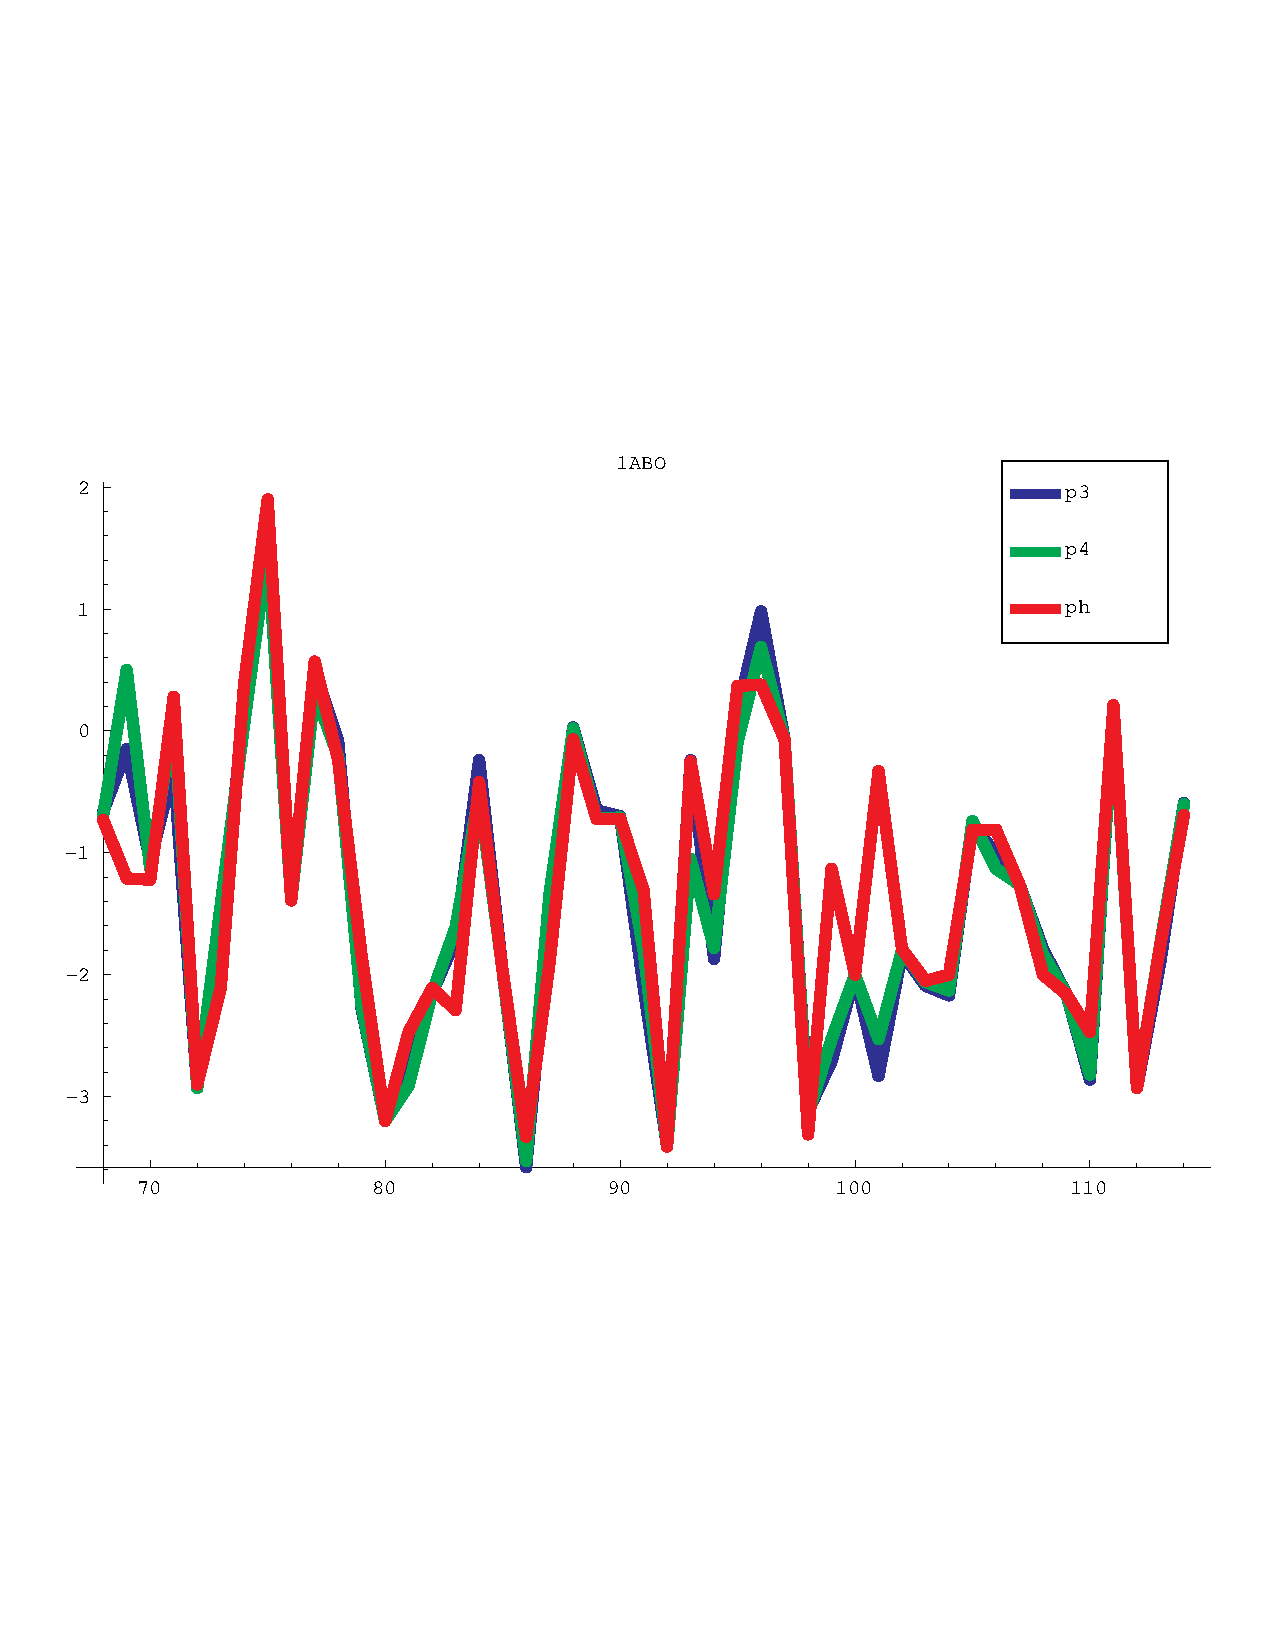
\includegraphics[trim=0cm 8cm 0cm 6cm,clip,width=8.5cm]{images/1ABO_simil_bypos.pdf} &
       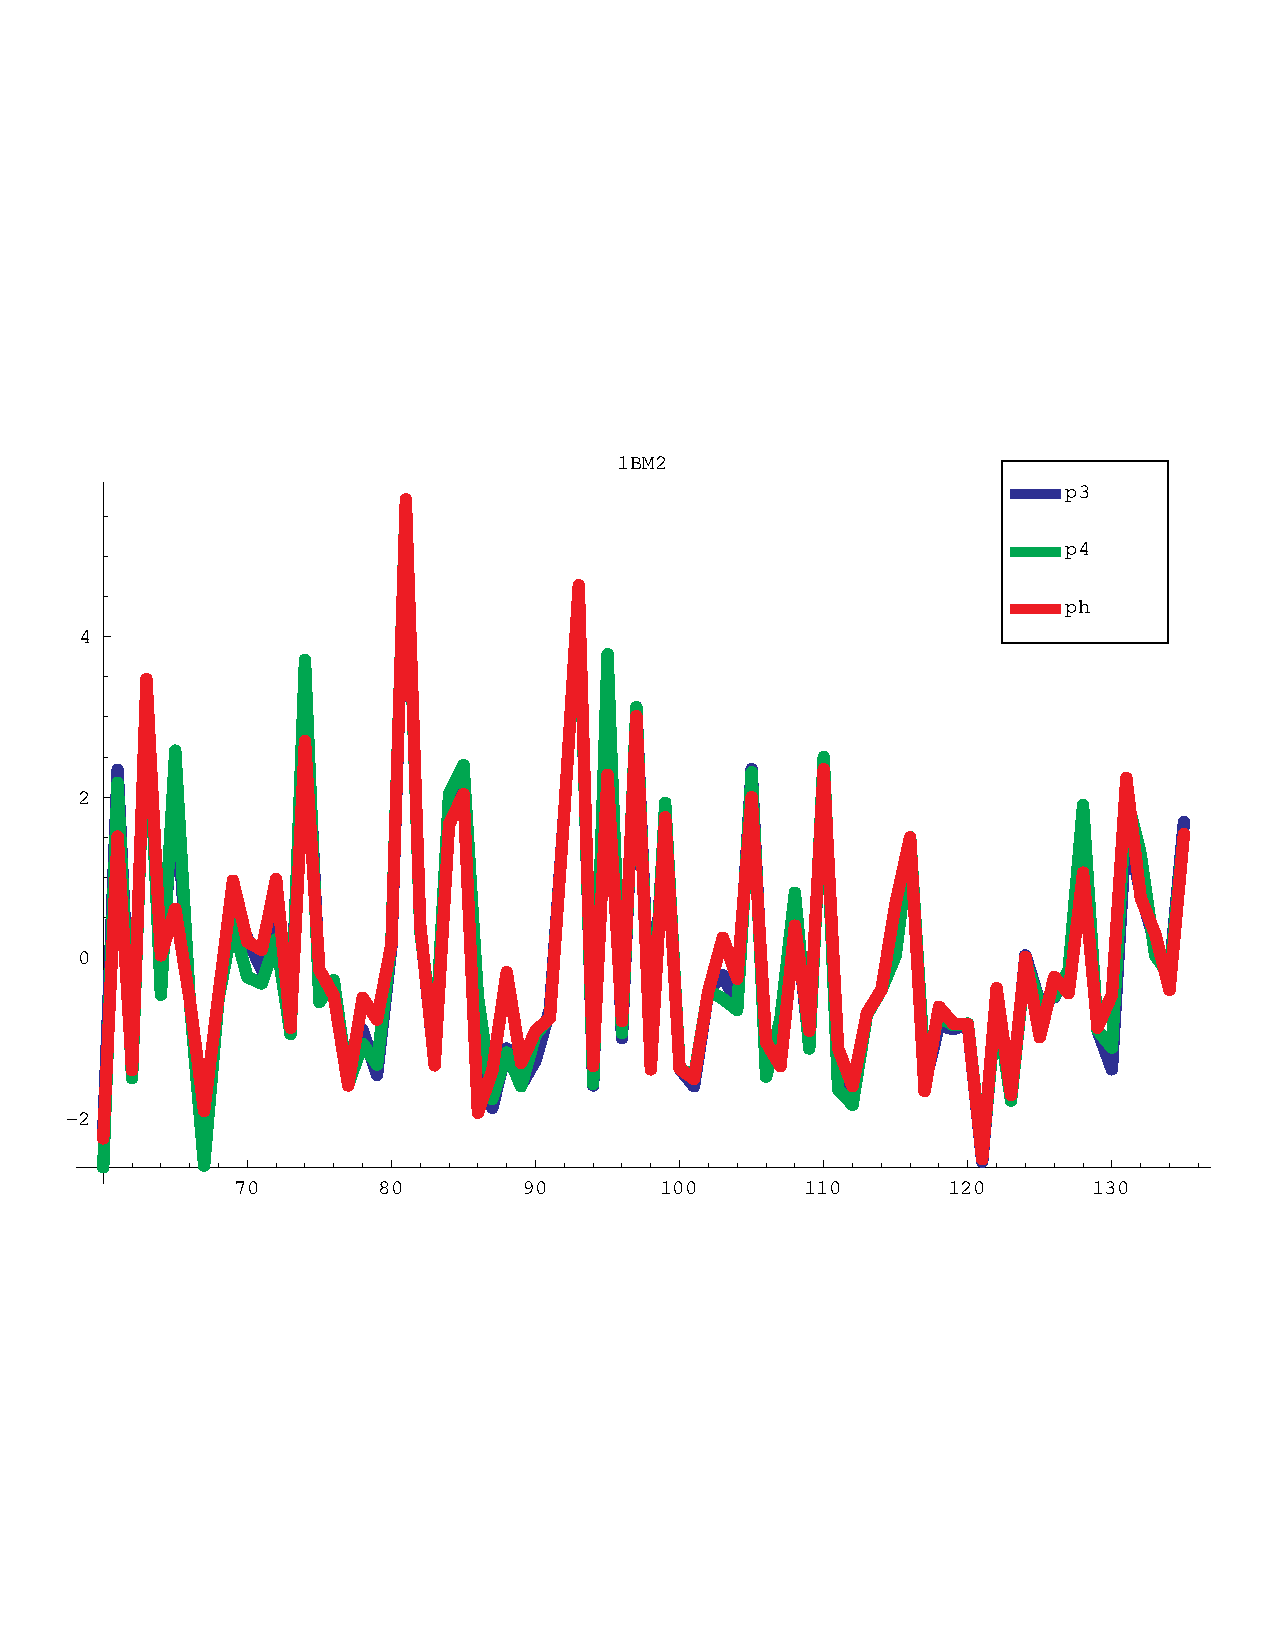
\includegraphics[trim=0cm 8cm 0cm 6cm,clip,width=8.5cm]{images/1BM2_simil_bypos.pdf} \\
       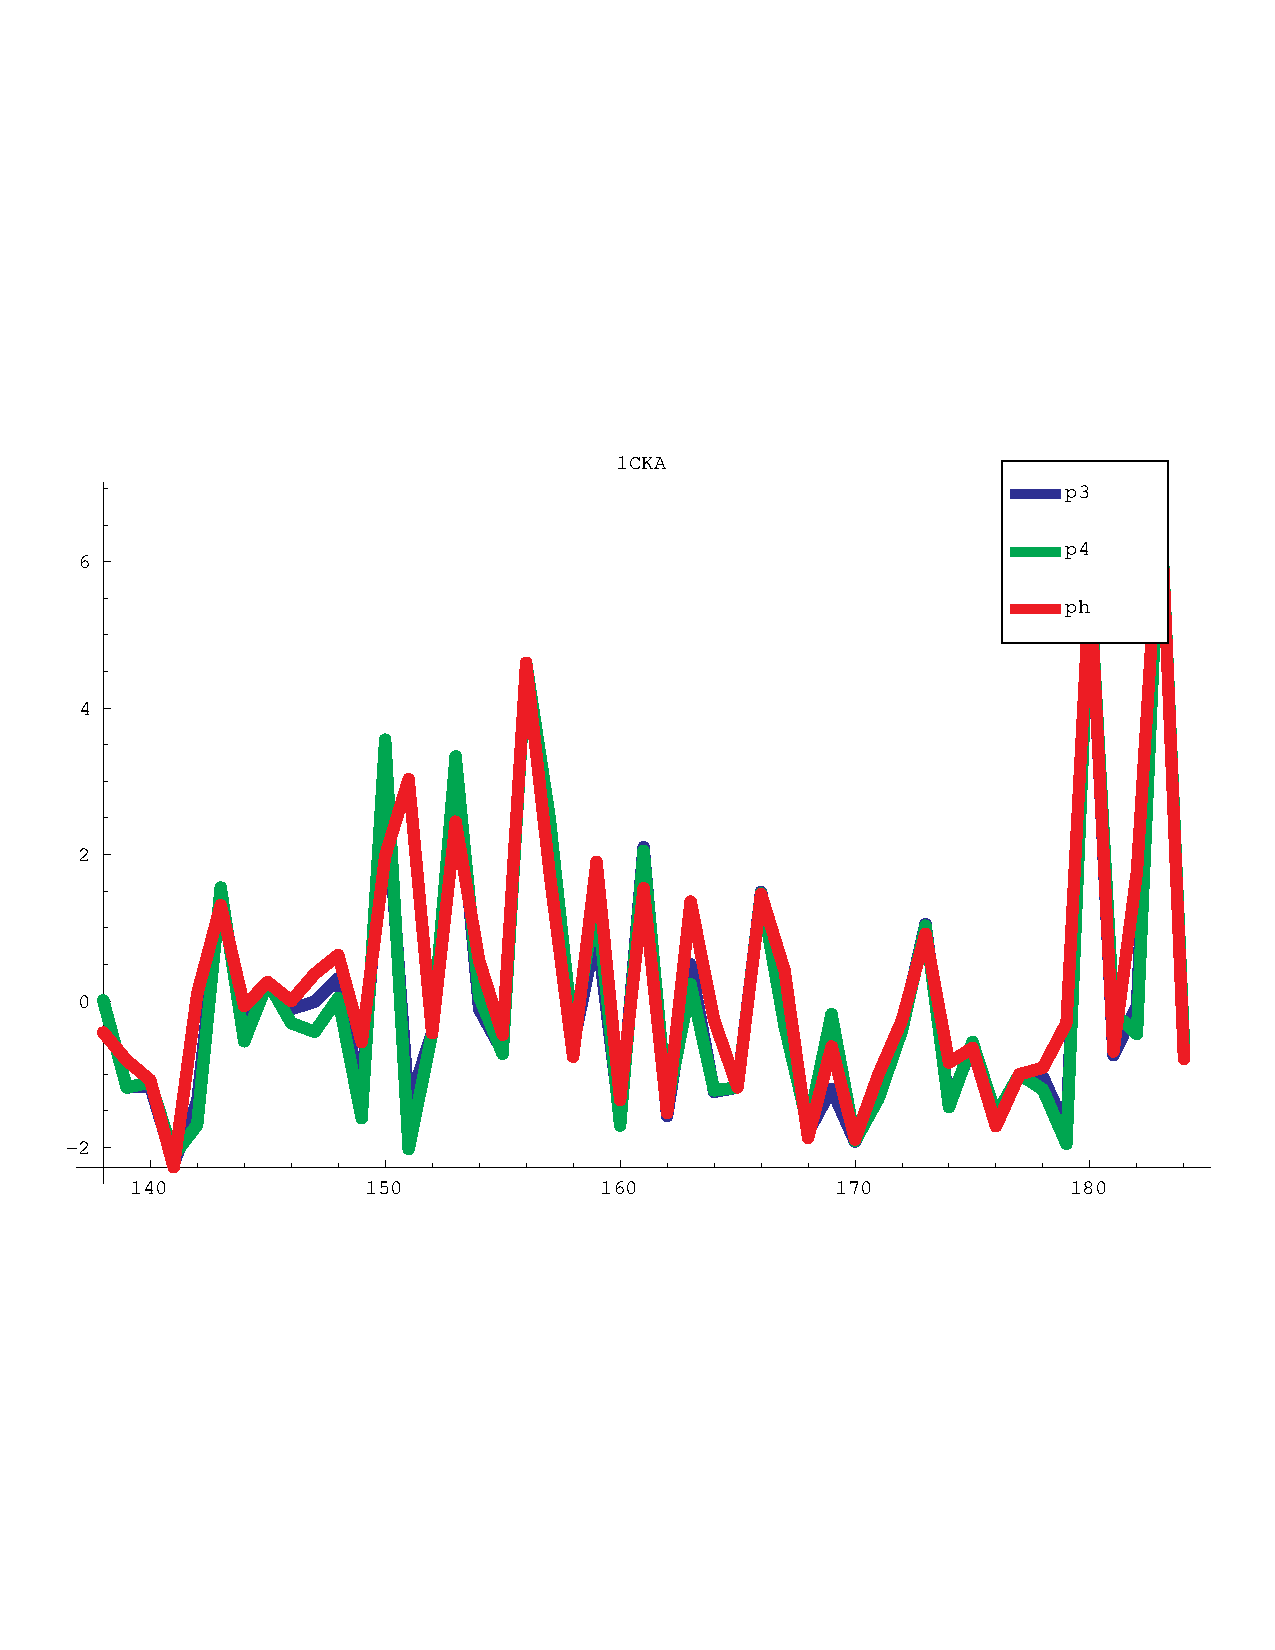
\includegraphics[trim=0cm 8cm 0cm 6cm,clip,width=8.5cm]{images/1CKA_simil_bypos.pdf} &
       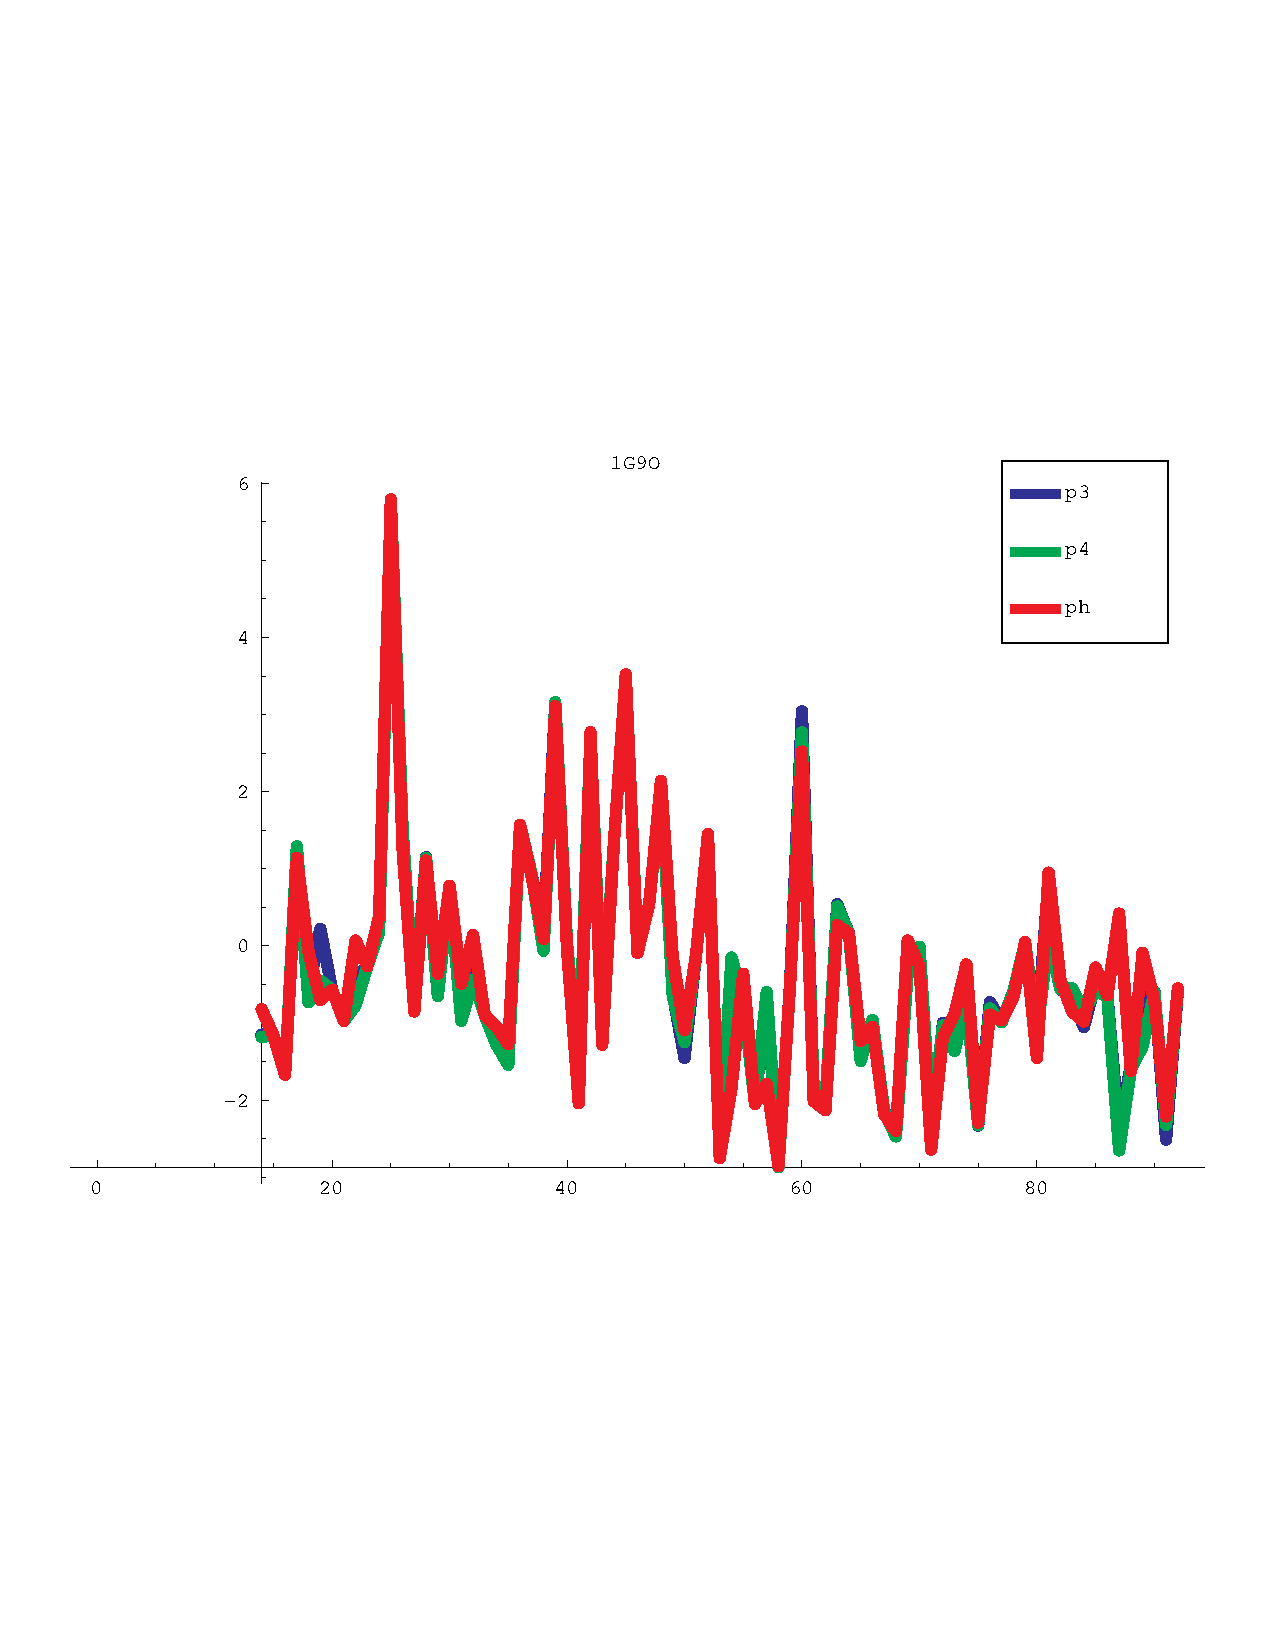
\includegraphics[trim=0cm 8cm 0cm 6cm,clip,width=8.5cm]{images/1G9O_simil_bypos.pdf} \\
       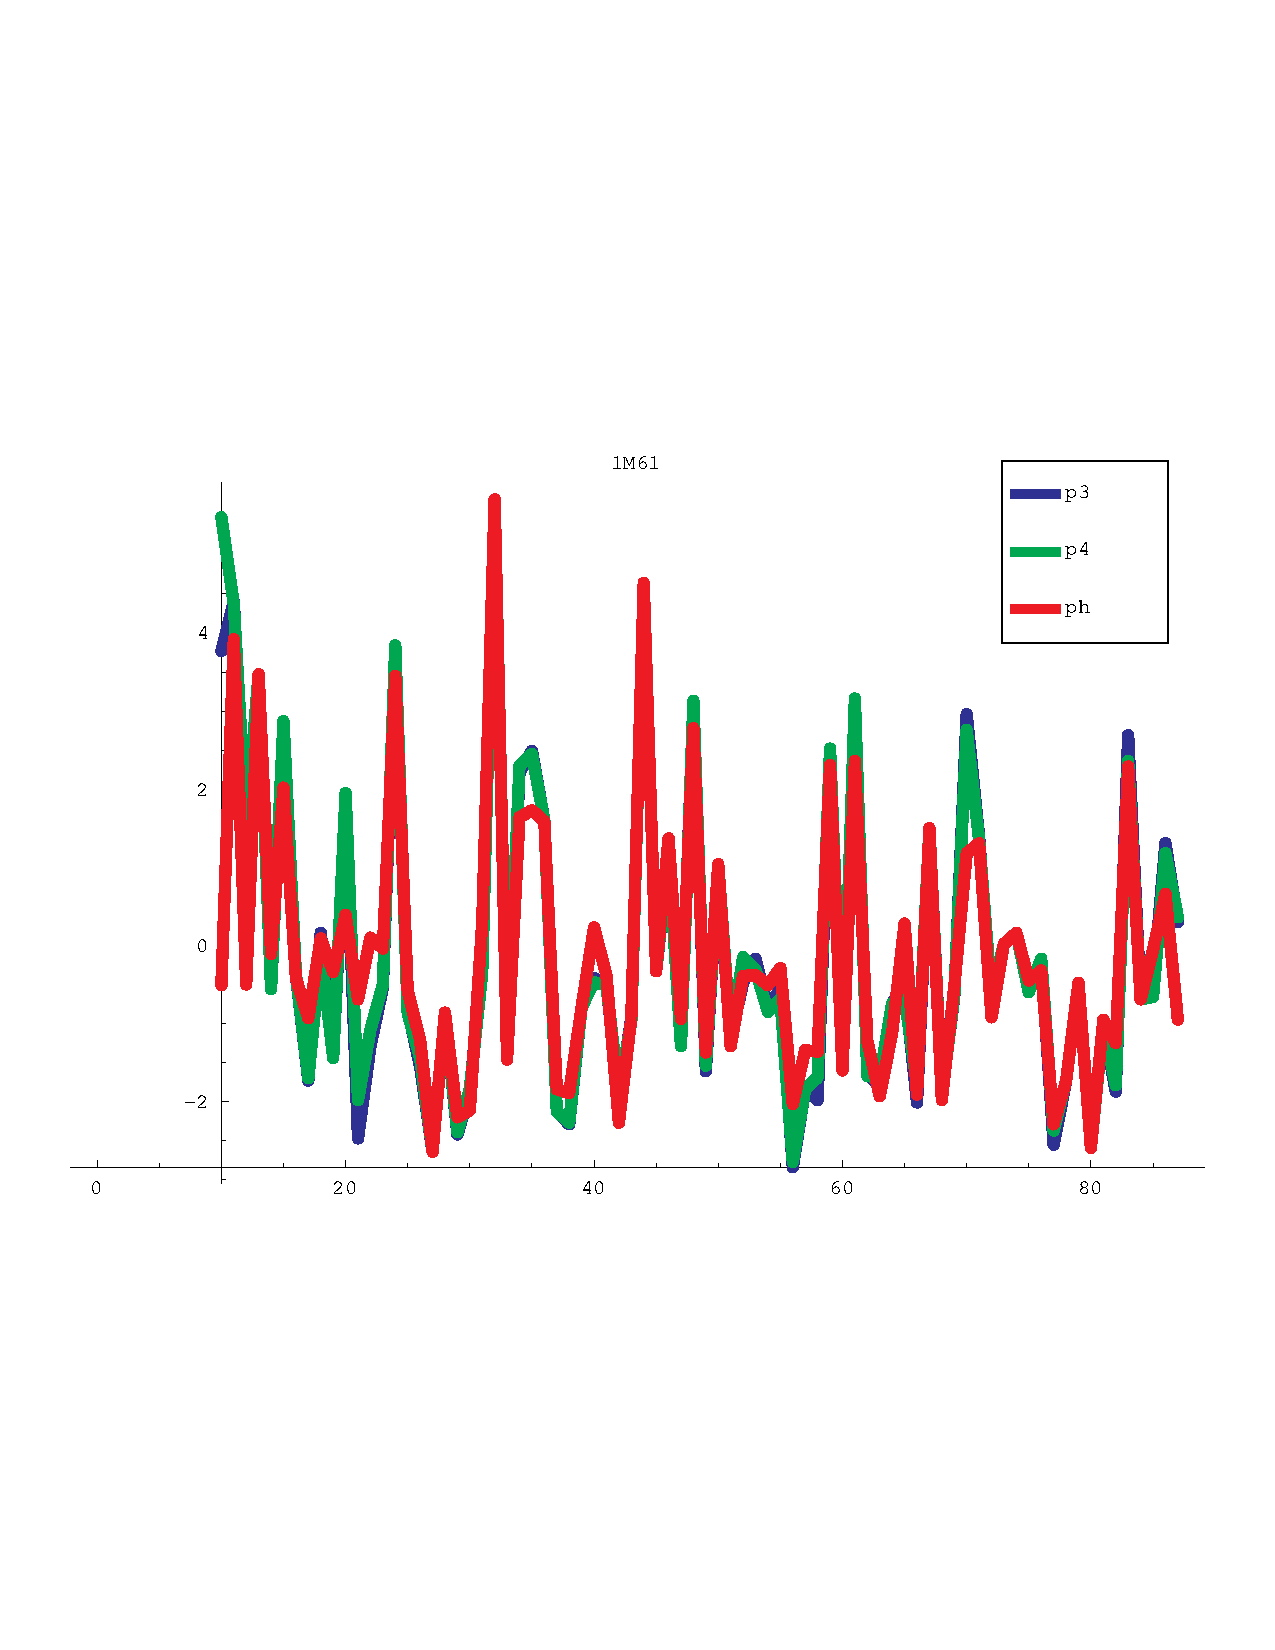
\includegraphics[trim=0cm 8cm 0cm 6cm,clip,width=8.5cm]{images/1M61_simil_bypos.pdf} &
       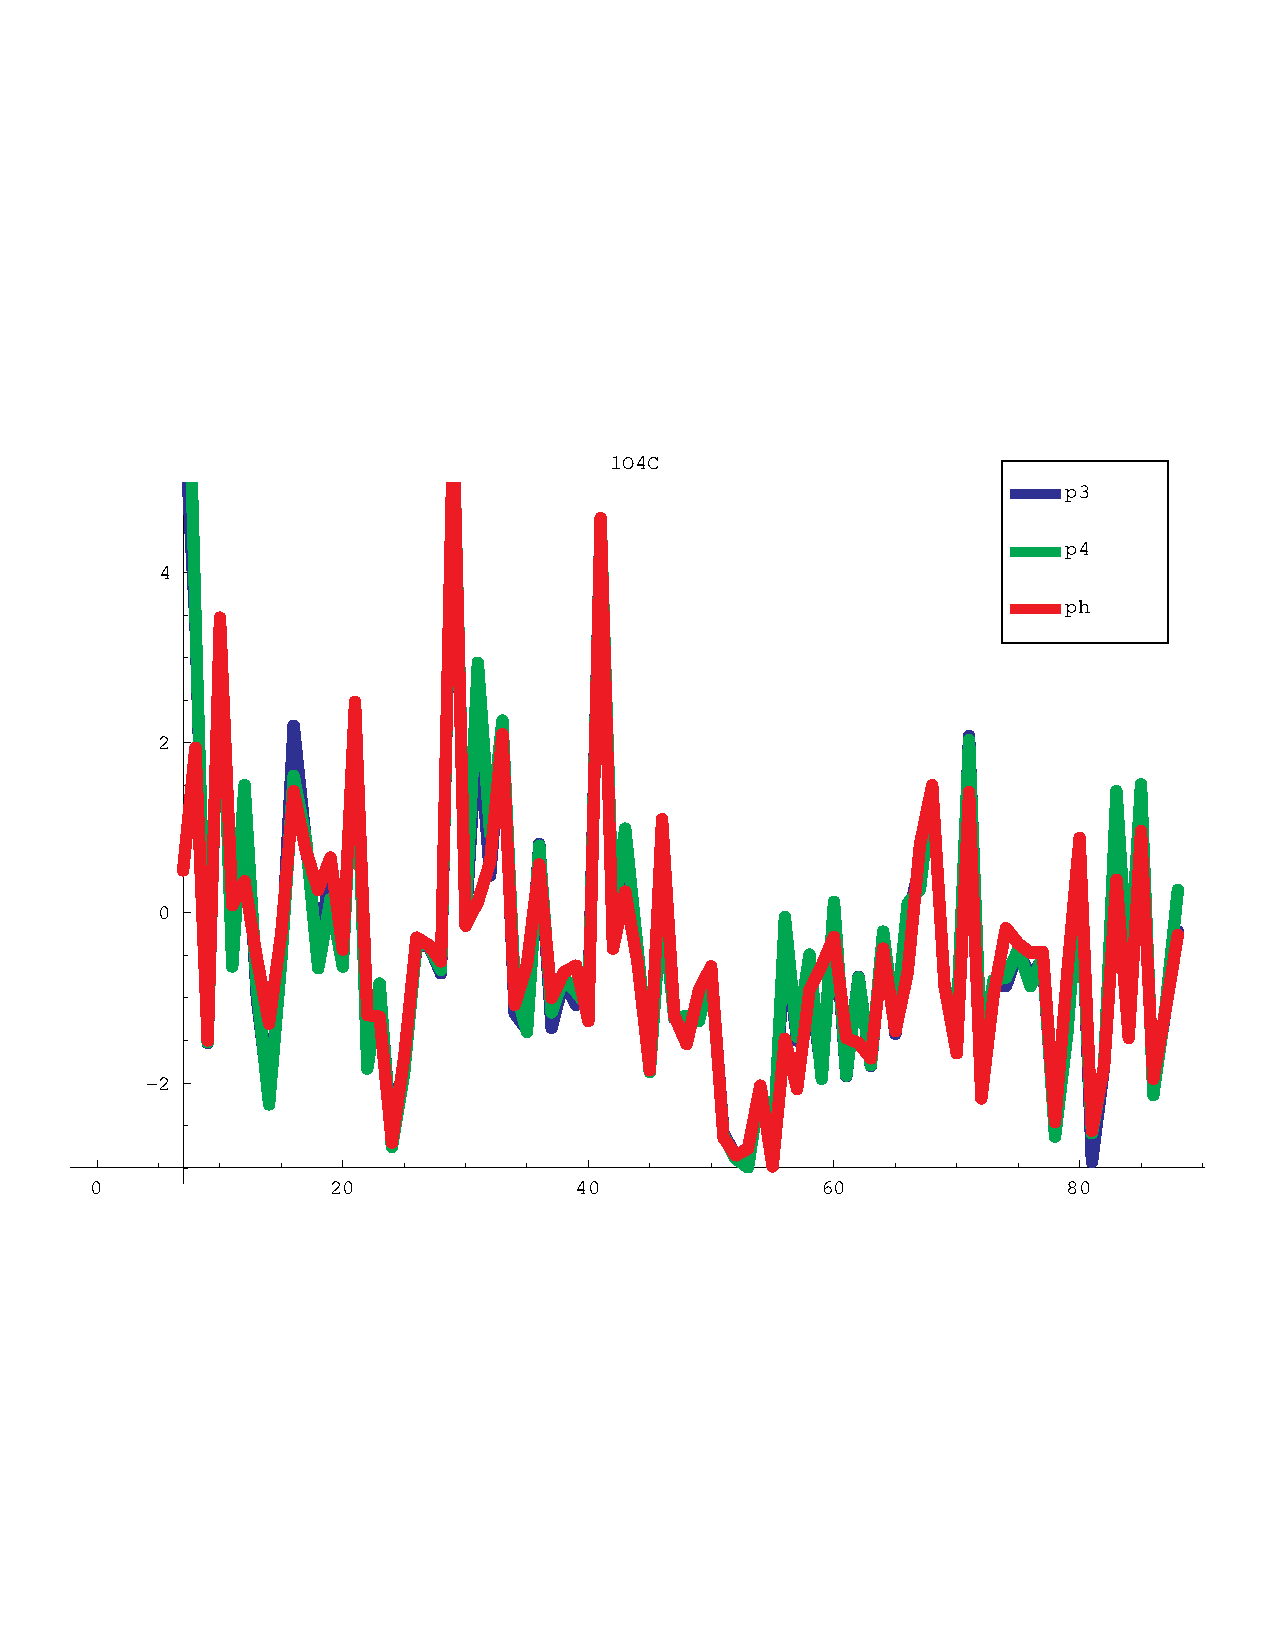
\includegraphics[trim=0cm 8cm 0cm 6cm,clip,width=8.5cm]{images/1O4C_simil_bypos.pdf} \\
       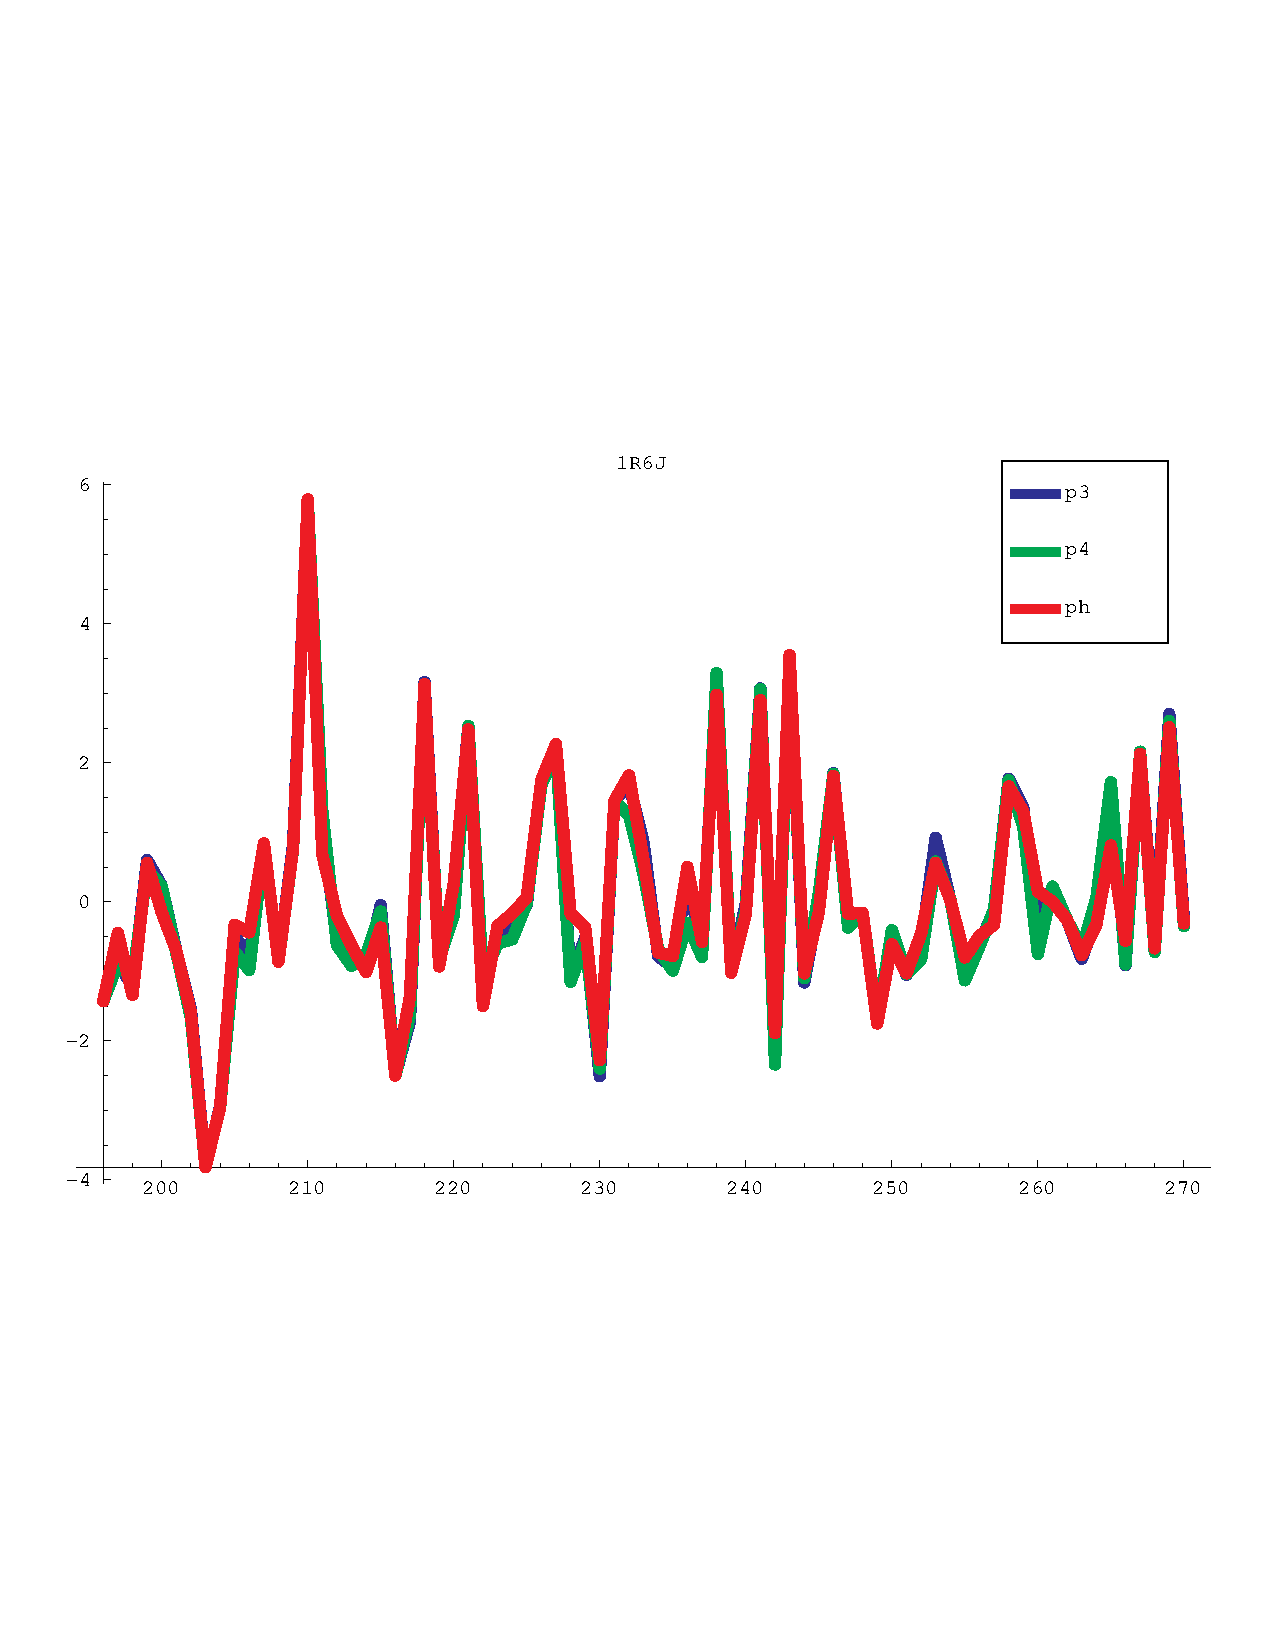
\includegraphics[trim=0cm 8cm 0cm 6cm,clip,width=8.5cm]{images/1R6J_simil_bypos.pdf} \\
     \end{tabular}
     
     \caption{Séquence logo et exponentiel de l'entropie pour une température de 0,3}
     \label{fig-seqlogo-T=03}
   \end{figure}

   \begin{figure}[t]
     \centering
     \begin{tabular}{cc}
       \includegraphics[width=8.45cm]{images/1ABO_p3_similarity_bypos.pdf} &
       \includegraphics[width=8.45cm]{images/1BM2_p3_similarity_bypos.pdf} \\
       \includegraphics[width=8.45cm]{images/1CKA_p3_similarity_bypos.pdf} &
       \includegraphics[width=8.45cm]{images/1G9O_p3_similarity_bypos.pdf} \\
       \includegraphics[width=8.45cm]{images/1M61_p3_similarity_bypos.pdf} &
       \includegraphics[width=8.45cm]{images/1O4C_p3_similarity_bypos.pdf} \\
       \includegraphics[width=8.45cm]{images/1R6J_p3_similarity_bypos.pdf} \\
     \end{tabular}
     
     \caption{Similarité par position pour le protocole p3.}
     \label{Sim_pos_byp3}
   \end{figure}
   \begin{figure}[t]
     \centering
     \begin{tabular}{cc}
       \includegraphics[width=8.45cm]{images/1ABO_p4_similarity_bypos.pdf} &
       \includegraphics[width=8.45cm]{images/1BM2_p4_similarity_bypos.pdf} \\
       \includegraphics[width=8.45cm]{images/1CKA_p4_similarity_bypos.pdf} &
       \includegraphics[width=8.45cm]{images/1G9O_p4_similarity_bypos.pdf} \\
       \includegraphics[width=8.45cm]{images/1M61_p4_similarity_bypos.pdf} &
       \includegraphics[width=8.45cm]{images/1O4C_p4_similarity_bypos.pdf} \\
       \includegraphics[width=8.45cm]{images/1R6J_p4_similarity_bypos.pdf} \\
     \end{tabular}
     
     \caption{Similarité par position pour le protocole p4.}
     \label{Sim_pos_byp4}
   \end{figure}
   \begin{figure}[t]
     \centering
     \begin{tabular}{cc}
       \includegraphics[width=8.45cm]{images/1ABO_ph_similarity_bypos.pdf} &
       \includegraphics[width=8.45cm]{images/1BM2_ph_similarity_bypos.pdf} \\
       \includegraphics[width=8.45cm]{images/1CKA_ph_similarity_bypos.pdf} &
       \includegraphics[width=8.45cm]{images/1G9O_ph_similarity_bypos.pdf} \\
       \includegraphics[width=8.45cm]{images/1M61_ph_similarity_bypos.pdf} &
       \includegraphics[width=8.45cm]{images/1O4C_ph_similarity_bypos.pdf} \\
       \includegraphics[width=8.45cm]{images/1R6J_ph_similarity_bypos.pdf} \\
     \end{tabular}
     
     \caption{Similarité par position pour le protocole ph.}
     \label{Sim_pos_byph}
   \end{figure}



   \begin{figure}[t]
     \centering
     \begin{tabular}{cc}
       \includegraphics[width=8.45cm]{images/1ABO_centiles.png} &
       \includegraphics[width=8.45cm]{images/1BM2_centiles.png} \\
       \includegraphics[width=8.45cm]{images/1CKA_centiles.png} &
       \includegraphics[width=8.45cm]{images/1G9O_centiles.png} \\
       \includegraphics[width=8.45cm]{images/1M61_centiles.png} &
       \includegraphics[width=8.45cm]{images/1O4C_centiles.png} \\
       \includegraphics[width=8.45cm]{images/1R6J_centiles.png} \\
     \end{tabular}
     
     \caption{Distribution des 100000 meilleurs séquences selon l'energie.}
     \label{fig-seqlogo-T=03}
   \end{figure}


 

\end{document}
